\documentclass[xcolor=svgnames,handout]{beamer}

\usepackage[utf8]    {inputenc}
\usepackage[T1]      {fontenc}
\usepackage[english] {babel}
\usepackage{graphicx}
\usepackage{listings}
\usepackage{fancyvrb}
\usepackage{amsmath,amsfonts,graphicx}
\usepackage{beamerleanprogress}


\title[End to end testing\hspace{2em}]{End to end testing and benchmarking of appliance disaggregation}

\author[Nithin Saji]{Nithin Saji\\{\small2010B5A7536P}}
%\date
\institute{BIDGELY}
\begin{document}
\maketitle


\section{The Objective}
\begin{frame}
An End to End Test runner that tests Bidgely's whole software and
hardware pipeline and generates comparisons with past perfomance as
well as ground truth.
\end{frame}

\section{Background}
\begin{frame}{What does Bidgely do ?}
  \begin{center}
    
\includegraphics[scale=0.5]{Bidgely-How-Much-Energy-Do-You-Use}
  \end{center}
\end{frame}

\begin{frame}{What does Bidgely do ?}
  \begin{center}
    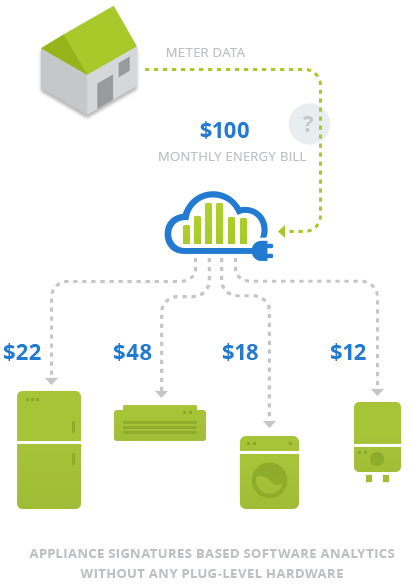
\includegraphics[scale=0.35]{bidgely_overview}
  \end{center}
\end{frame}



\begin{frame}
  \frametitle{What is Disaggregation?}

  The process of analyzing changes in consumption of a home to deduce
  the appliances used and the individual energy consumption.

  \begin{itemize}
  \item Input: a data stream of household electricity usage from a single
    point (e.g.smart meter data, gateway)
  \item External input: Weather, temperature etc.
  \item Output: Amount of consumption of each major Appliance.
  \end{itemize}
\end{frame}


\begin{frame}
How does that work?
\end{frame}

\begin{frame}{Collect Data}
  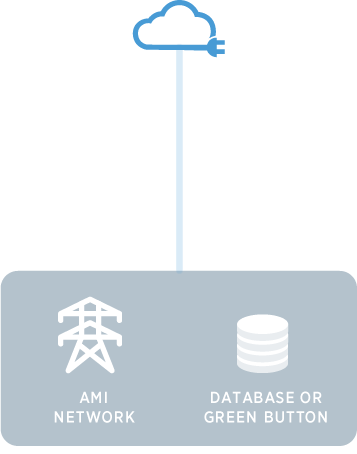
\includegraphics[width=0.45\textwidth]{technology_workds_with_ami}
  \hfill
  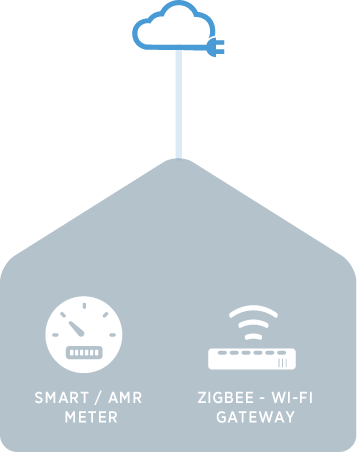
\includegraphics[width=0.45\textwidth]{technology_workds_with_han}
\end{frame}


\begin{frame}{Learn from Data}
  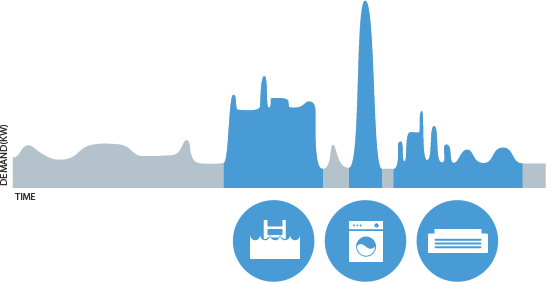
\includegraphics[width=0.4\textwidth]{technology_algorithms_work}
  \hfill
  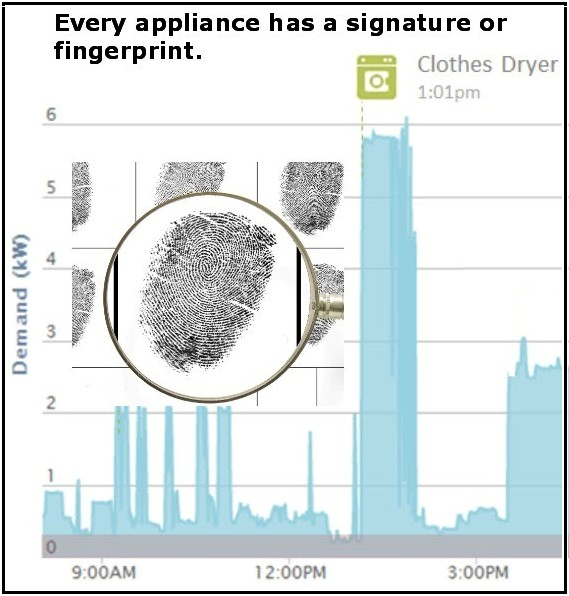
\includegraphics[width=0.4\textwidth]{appliance-signature}
\end{frame}

\begin{frame}{How to test and benchmark?}
  An end to end tester for comparing results and ground truth.
\end{frame}


\section
    {Methodology}

    \begin{frame}
      {End to End Tester}
      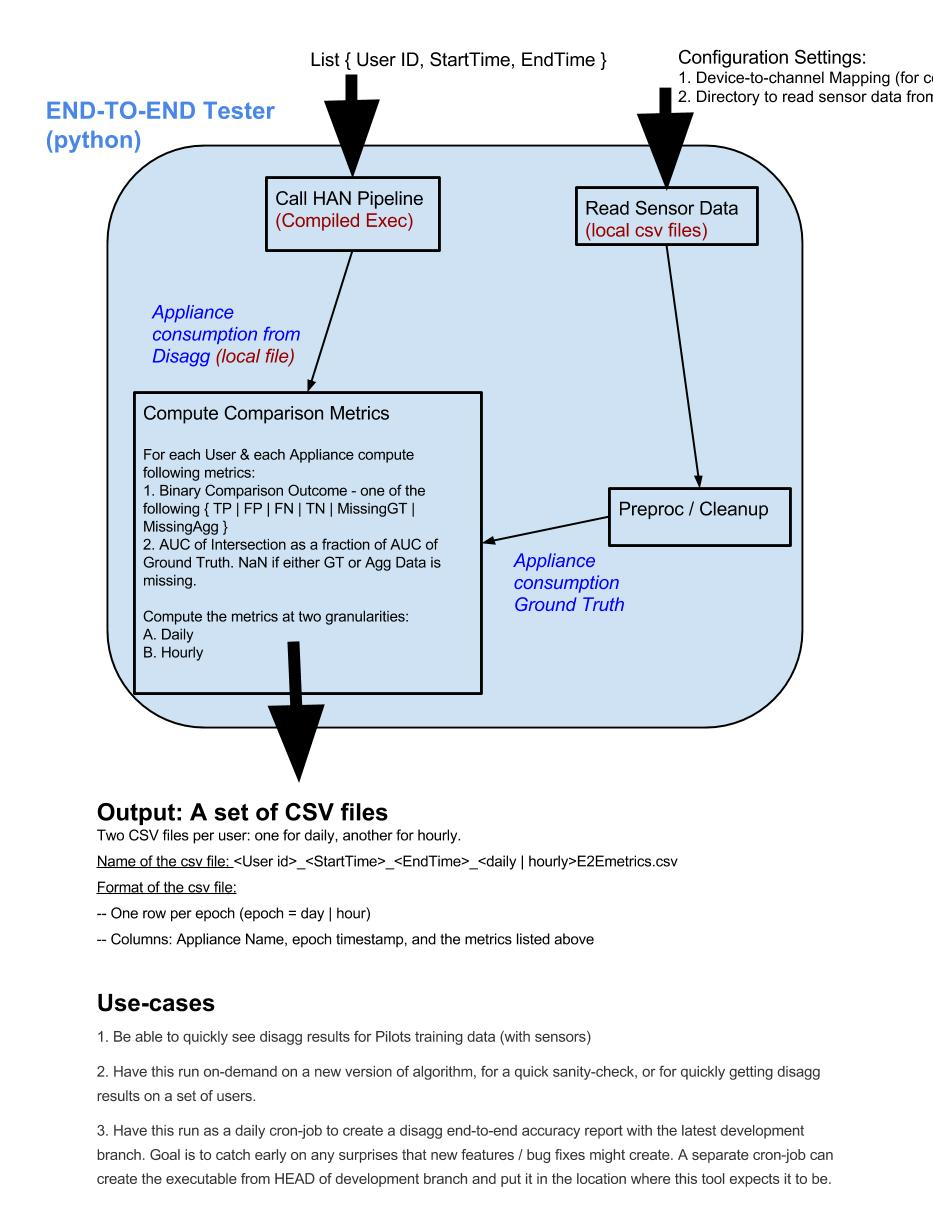
\includegraphics[height=\textheight]{Design_of_End2End_tester}
    \end{frame}


    \begin{frame}
      {How HAN works}

      \begin{figure}[t]
        \centering
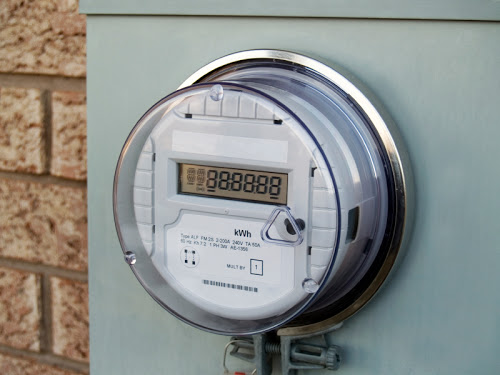
\includegraphics[width=0.45\textwidth]{Smart-Meters1}
\hfill
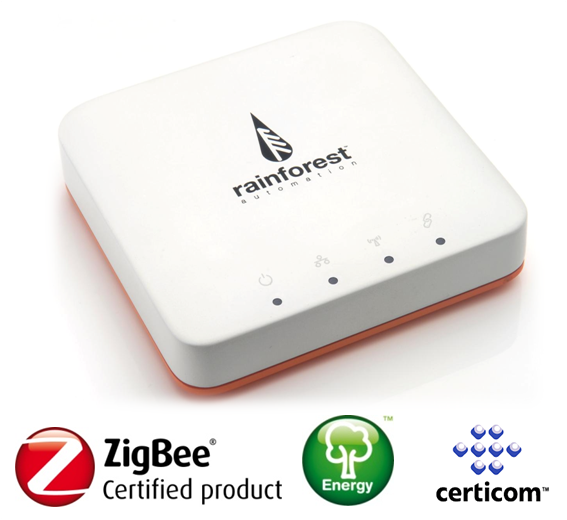
\includegraphics[width=0.45\textwidth]{eagle-picture}
        \caption{Smart Energy Meter and Gateway Device}
      \end{figure}
    \end{frame}


    \begin{frame}
      {Plug level Sensors}
      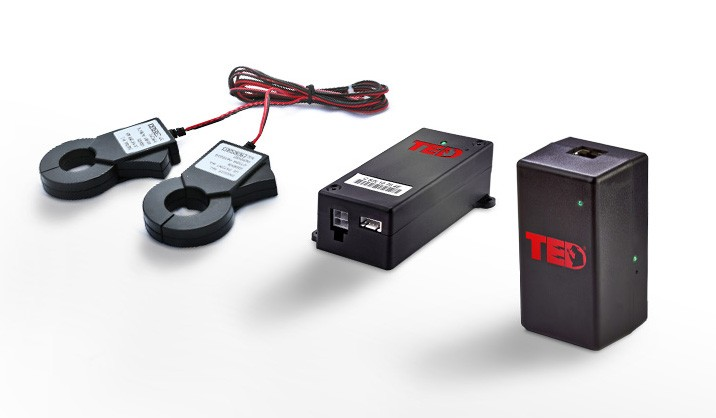
\includegraphics[width=0.5\textwidth]{package_wo_handset}
      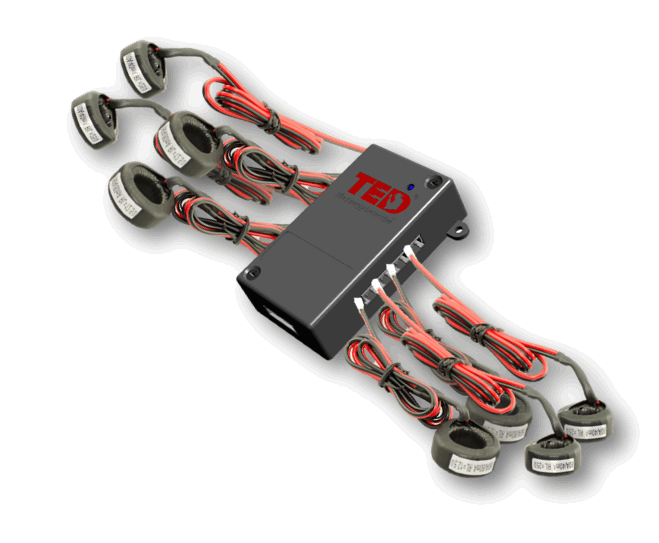
\includegraphics[width=0.5\textwidth]{spyder}
    \end{frame}

    \begin{frame}{End to End Tester design}
      \begin{itemize}
      \item The tool accepts csv with the user id's and the timestamp
        to run the tests
        \pause
      \item sensor vs  han pipeline exec output
        \pause
      \item sensor vs disagg from api
        \pause
      \item hanpipeline exec output vs disagg from api
        \pause
      \item hanpipeline exec output vs hanpipeline exec output
        \pause
      \item disagg api vs disagg api
        \pause

      \end{itemize}
      
    \end{frame}

    \begin{frame}{Syncing data}
       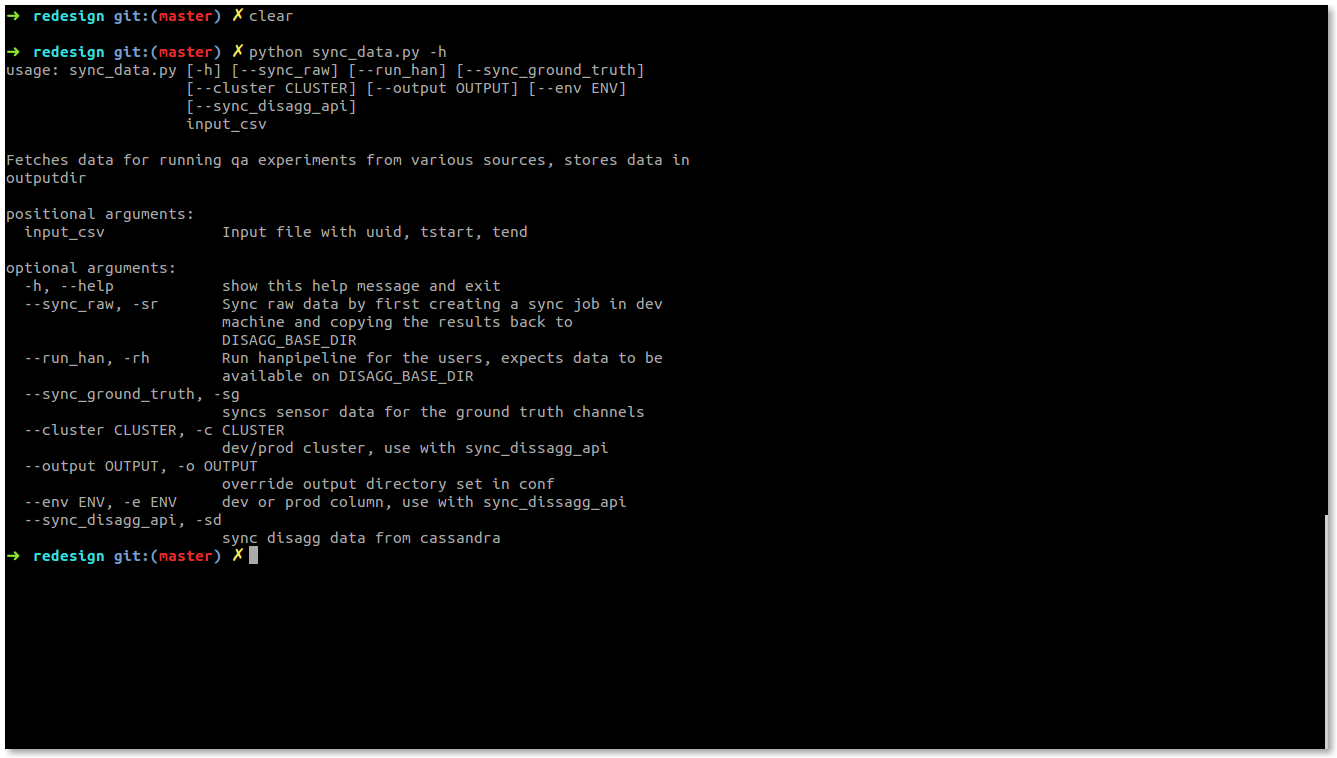
\includegraphics[height=0.8\textheight]{sync}
    \end{frame}
    
    
    \begin{frame}{Generating metrics}
      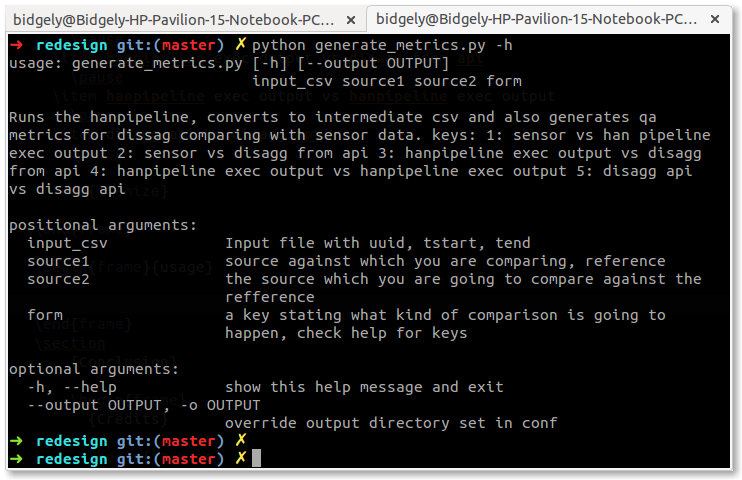
\includegraphics[height=0.8\textheight]{usage}
    \end{frame}

    \section{Results and Analysis}
    \begin{frame}{Results}
      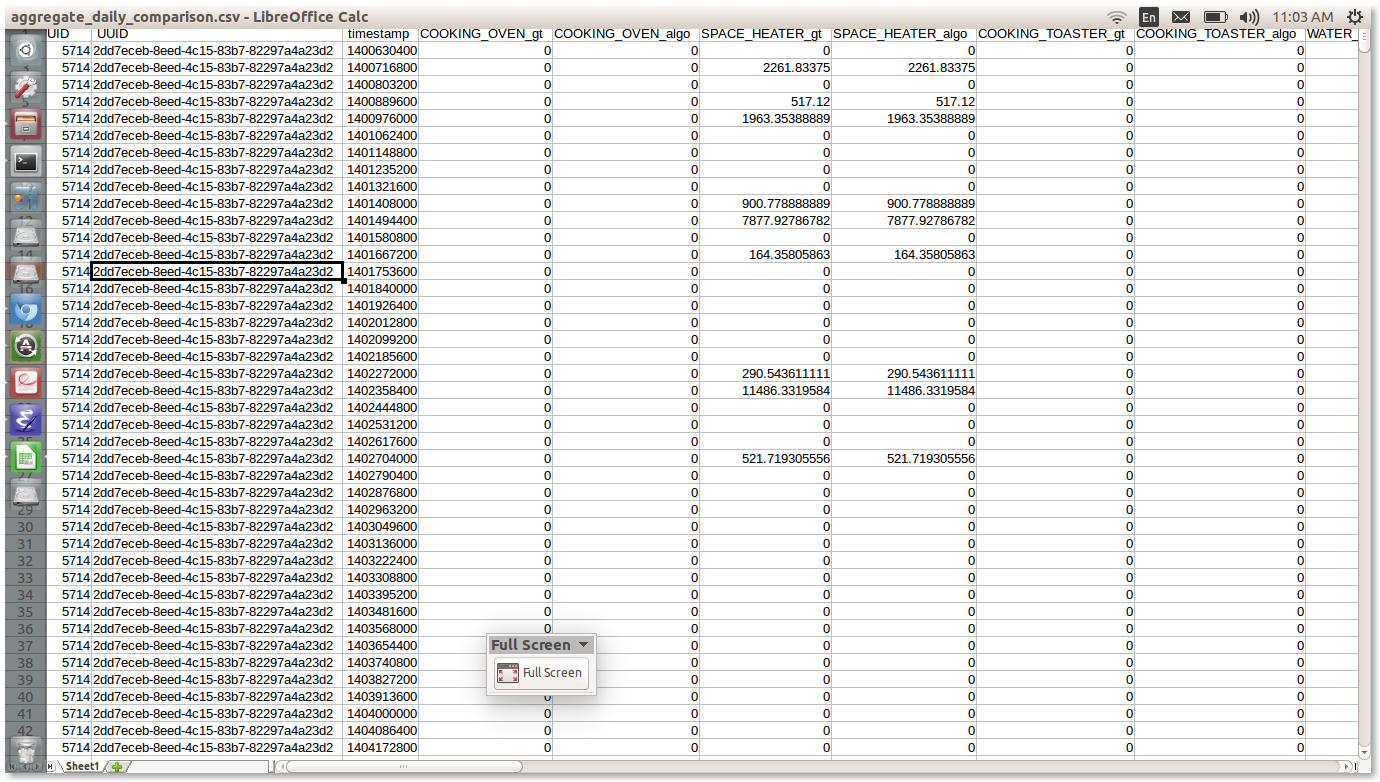
\includegraphics[width=0.8\textwidth]{aggregate}
    \end{frame}
    \begin{frame}{Binary comparison aggregate for a user}
      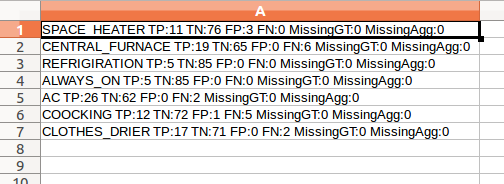
\includegraphics[width=0.8\textwidth]{result_binary}
    \end{frame}
    \begin{frame}{Daily stats for a user}
      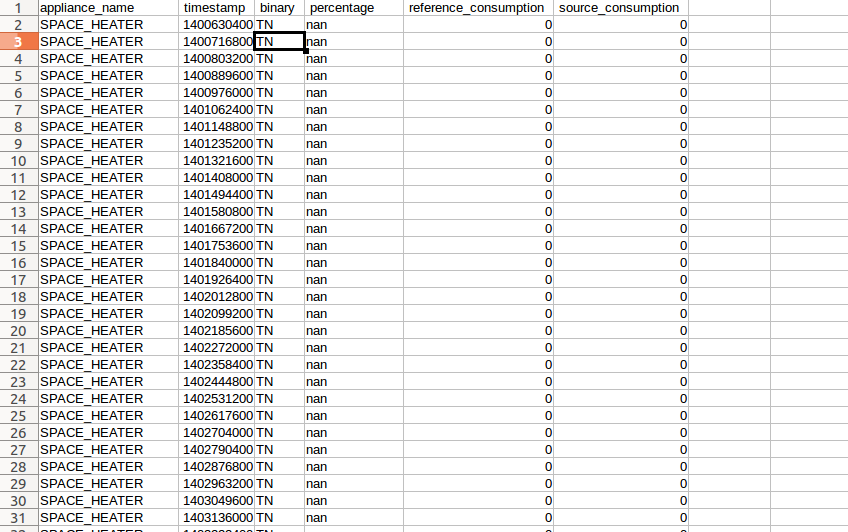
\includegraphics[width=0.8\textwidth]{results_daily}
    \end{frame}
    
    \section{Post Mid Sem}
    \begin{frame}{Current status and post midsem plans}
      \begin{itemize}
        \item Bug fixes for the end to end tester.
        \item A testing Suite for gateway devices.
        \item A Simulation Suite for creating mock data , to be used with
          end to end tester
      \end{itemize}

    \end{frame}
    
    \begin{frame}
      {Test Suite for Gateway Device}
      \begin{itemize}
      \item Create mock data and feed it to a smart meter simulator.
      \item Connect to the meter over serial interface and check
        whether the data matches or not.
      \item Poll the cloud api's to make sure that the data is sent to
        cloud,
      \item Create a comandline interface for doing all of this.
      \end{itemize}
    \end{frame}

    \begin{frame}
      {Simulation Suite}
      \begin{itemize}
      \item Bidgely doesn't have too many houses with plug level
        sensors.
      \item The data from the available plug level sensors are often
        contaminated.
      \item Can the data be simulated?
      \end{itemize}
    \end{frame}

    \begin{frame}{The Plan}
      \begin{itemize}
      \item Model different appliances from the available data.
      \item The model should be designed to be tweakable to simulate
        different variations of appliances.
      \item The simulated appliances could be added up to simulate a
        house's load signal.
      \end{itemize}
    \end{frame}
    \section
        {Summary and Conclusion}

        \begin{frame}
          {Summary}

          \begin{itemize}
          \item Build a tool for comparing ground truth to the
            disaggregation results.
          \item Built tools for automating data fetching for testing
            and benchmarking.
          \item Automate more things in the future.
          \end{itemize}
        \end{frame}


        \begin{frame}
          {Questions}
        \end{frame}

\end{document}

